
\documentclass[12pt]{article}
\usepackage{fancyhdr}
\renewcommand{\familydefault}{\sfdefault}
\renewcommand*{\ttdefault}{\familydefault}
\usepackage[paperwidth=35cm,paperheight=50cm,left =1cm, top = 1cm, right =1cm, bottom = 1cm ,marginparwidth=0cm, includeheadfoot,headheight=66pt, headsep=0cm]{geometry}
\usepackage{pgfplots}
\pgfplotsset{width=5cm,compat=newest}
\usetikzlibrary{plotmarks}
\usepgfplotslibrary{dateplot}
\usepgfplotslibrary{units}
\tikzset{every picture/.append style={font=\normalsize}} % size graph font
\usetikzlibrary{arrows, positioning, calc}

\tikzstyle{chart}=[
legend label/.style={font={\Large},anchor=west,align=left},
legend box/.style={rectangle, draw, minimum size=5pt},
axis/.style={black,semithick,->},
axis label/.style={anchor=east,font={\tiny}}]

\definecolor{customcolor}{HTML}{1d5893}
\begin{document}
\begin{minipage}{0.96\linewidth}
\flushleft
\begin{tikzpicture}
\pgfplotscreateplotcyclelist{defaultCycle}{%
ybar,%ybar legend,
fill=customcolor,draw=black,opacity=1,thin,solid,mark=no,mark options=solid,\\%
}


    
\begin{axis}
[
    cycle list name=defaultCycle,
    width=0.8\linewidth,
    height=0.15\textheight,
    use units,
    scale only axis,
    symbolic x coords={},
    xtick=data,
    nodes near coords,
    yticklabel style={/pgf/number format/fixed},
    ytick pos=left,
    axis y line*=left,
    xtick pos=bottom,
    axis x line*=bottom,
    legend style={draw=none,at={(0,1.03)},anchor=south west},
    legend columns=-1,
    xtick align=center,
    ytick align=center,
    xtick distance=0.1,
    ytick distance=,
    x tick label style ={font=\normalsize,text width=0.3cm,anchor=north,rotate=0,align=center},
    y tick label style ={font=\normalsize,text width=2cm,anchor=east,rotate=0,align=right},
    scaled y ticks=false,
    bar width=35pt,
    ymajorgrids,
    ylabel=\textbf{Number of Hours Worked},
    xlabel=\textbf{Task Name},
    title=\textbf Tugman{'s Work Week Breakdown},
    ,
    ]

    \addplot  + table [x={x},y={y},meta index=2,col sep=comma] {
    x, y, z
    };

\end{axis}
\end{tikzpicture}
\end{minipage}

\newpage



    
\begin{axis}
[
    cycle list name=defaultCycle,
    width=0.8\linewidth,
    height=0.15\textheight,
    use units,
    scale only axis,
    symbolic x coords={},
    xtick=data,
    nodes near coords,
    yticklabel style={/pgf/number format/fixed},
    ytick pos=left,
    axis y line*=left,
    xtick pos=bottom,
    axis x line*=bottom,
    legend style={draw=none,at={(0,1.03)},anchor=south west},
    legend columns=-1,
    xtick align=center,
    ytick align=center,
    xtick distance=0.1,
    ytick distance=,
    x tick label style ={font=\normalsize,text width=0.3cm,anchor=north,rotate=0,align=center},
    y tick label style ={font=\normalsize,text width=2cm,anchor=east,rotate=0,align=right},
    scaled y ticks=false,
    bar width=35pt,
    ymajorgrids,
    ylabel=\textbf{Number of Hours Worked},
    xlabel=\textbf{Task Name},
    title=\textbf monica {'s Work Week Breakdown},
    ,
    ]

    \addplot  + table [x={x},y={y},meta index=2,col sep=comma] {
    x, y, z
    };

\end{axis}
\end{tikzpicture}
\end{minipage}

\newpage



    
\begin{axis}
[
    cycle list name=defaultCycle,
    width=0.8\linewidth,
    height=0.15\textheight,
    use units,
    scale only axis,
    symbolic x coords={},
    xtick=data,
    nodes near coords,
    yticklabel style={/pgf/number format/fixed},
    ytick pos=left,
    axis y line*=left,
    xtick pos=bottom,
    axis x line*=bottom,
    legend style={draw=none,at={(0,1.03)},anchor=south west},
    legend columns=-1,
    xtick align=center,
    ytick align=center,
    xtick distance=0.1,
    ytick distance=,
    x tick label style ={font=\normalsize,text width=0.3cm,anchor=north,rotate=0,align=center},
    y tick label style ={font=\normalsize,text width=2cm,anchor=east,rotate=0,align=right},
    scaled y ticks=false,
    bar width=35pt,
    ymajorgrids,
    ylabel=\textbf{Number of Hours Worked},
    xlabel=\textbf{Task Name},
    title=\textbf Sam{'s Work Week Breakdown},
    ,
    ]

    \addplot  + table [x={x},y={y},meta index=2,col sep=comma] {
    x, y, z
    };

\end{axis}
\end{tikzpicture}
\end{minipage}

\newpage



    
\begin{axis}
[
    cycle list name=defaultCycle,
    width=0.8\linewidth,
    height=0.15\textheight,
    use units,
    scale only axis,
    symbolic x coords={},
    xtick=data,
    nodes near coords,
    yticklabel style={/pgf/number format/fixed},
    ytick pos=left,
    axis y line*=left,
    xtick pos=bottom,
    axis x line*=bottom,
    legend style={draw=none,at={(0,1.03)},anchor=south west},
    legend columns=-1,
    xtick align=center,
    ytick align=center,
    xtick distance=0.1,
    ytick distance=,
    x tick label style ={font=\normalsize,text width=0.3cm,anchor=north,rotate=0,align=center},
    y tick label style ={font=\normalsize,text width=2cm,anchor=east,rotate=0,align=right},
    scaled y ticks=false,
    bar width=35pt,
    ymajorgrids,
    ylabel=\textbf{Number of Hours Worked},
    xlabel=\textbf{Task Name},
    title=\textbf Michelle{'s Work Week Breakdown},
    ,
    ]

    \addplot  + table [x={x},y={y},meta index=2,col sep=comma] {
    x, y, z
    };

\end{axis}
\end{tikzpicture}
\end{minipage}

\newpage



    
\begin{axis}
[
    cycle list name=defaultCycle,
    width=0.8\linewidth,
    height=0.15\textheight,
    use units,
    scale only axis,
    symbolic x coords={},
    xtick=data,
    nodes near coords,
    yticklabel style={/pgf/number format/fixed},
    ytick pos=left,
    axis y line*=left,
    xtick pos=bottom,
    axis x line*=bottom,
    legend style={draw=none,at={(0,1.03)},anchor=south west},
    legend columns=-1,
    xtick align=center,
    ytick align=center,
    xtick distance=0.1,
    ytick distance=,
    x tick label style ={font=\normalsize,text width=0.3cm,anchor=north,rotate=0,align=center},
    y tick label style ={font=\normalsize,text width=2cm,anchor=east,rotate=0,align=right},
    scaled y ticks=false,
    bar width=35pt,
    ymajorgrids,
    ylabel=\textbf{Number of Hours Worked},
    xlabel=\textbf{Task Name},
    title=\textbf Nickole{'s Work Week Breakdown},
    ,
    ]

    \addplot  + table [x={x},y={y},meta index=2,col sep=comma] {
    x, y, z
    };

\end{axis}
\end{tikzpicture}
\end{minipage}

\newpage



    
\begin{axis}
[
    cycle list name=defaultCycle,
    width=0.8\linewidth,
    height=0.15\textheight,
    use units,
    scale only axis,
    symbolic x coords={},
    xtick=data,
    nodes near coords,
    yticklabel style={/pgf/number format/fixed},
    ytick pos=left,
    axis y line*=left,
    xtick pos=bottom,
    axis x line*=bottom,
    legend style={draw=none,at={(0,1.03)},anchor=south west},
    legend columns=-1,
    xtick align=center,
    ytick align=center,
    xtick distance=0.1,
    ytick distance=,
    x tick label style ={font=\normalsize,text width=0.3cm,anchor=north,rotate=0,align=center},
    y tick label style ={font=\normalsize,text width=2cm,anchor=east,rotate=0,align=right},
    scaled y ticks=false,
    bar width=35pt,
    ymajorgrids,
    ylabel=\textbf{Number of Hours Worked},
    xlabel=\textbf{Task Name},
    title=\textbf Kristen{'s Work Week Breakdown},
    ,
    ]

    \addplot  + table [x={x},y={y},meta index=2,col sep=comma] {
    x, y, z
    };

\end{axis}
\end{tikzpicture}
\end{minipage}

\newpage



    
\begin{axis}
[
    cycle list name=defaultCycle,
    width=0.8\linewidth,
    height=0.15\textheight,
    use units,
    scale only axis,
    symbolic x coords={},
    xtick=data,
    nodes near coords,
    yticklabel style={/pgf/number format/fixed},
    ytick pos=left,
    axis y line*=left,
    xtick pos=bottom,
    axis x line*=bottom,
    legend style={draw=none,at={(0,1.03)},anchor=south west},
    legend columns=-1,
    xtick align=center,
    ytick align=center,
    xtick distance=0.1,
    ytick distance=,
    x tick label style ={font=\normalsize,text width=0.3cm,anchor=north,rotate=0,align=center},
    y tick label style ={font=\normalsize,text width=2cm,anchor=east,rotate=0,align=right},
    scaled y ticks=false,
    bar width=35pt,
    ymajorgrids,
    ylabel=\textbf{Number of Hours Worked},
    xlabel=\textbf{Task Name},
    title=\textbf Paul {'s Work Week Breakdown},
    ,
    ]

    \addplot  + table [x={x},y={y},meta index=2,col sep=comma] {
    x, y, z
    };

\end{axis}
\end{tikzpicture}
\end{minipage}

\newpage



    
\begin{axis}
[
    cycle list name=defaultCycle,
    width=0.8\linewidth,
    height=0.15\textheight,
    use units,
    scale only axis,
    symbolic x coords={},
    xtick=data,
    nodes near coords,
    yticklabel style={/pgf/number format/fixed},
    ytick pos=left,
    axis y line*=left,
    xtick pos=bottom,
    axis x line*=bottom,
    legend style={draw=none,at={(0,1.03)},anchor=south west},
    legend columns=-1,
    xtick align=center,
    ytick align=center,
    xtick distance=0.1,
    ytick distance=,
    x tick label style ={font=\normalsize,text width=0.3cm,anchor=north,rotate=0,align=center},
    y tick label style ={font=\normalsize,text width=2cm,anchor=east,rotate=0,align=right},
    scaled y ticks=false,
    bar width=35pt,
    ymajorgrids,
    ylabel=\textbf{Number of Hours Worked},
    xlabel=\textbf{Task Name},
    title=\textbf Todd{'s Work Week Breakdown},
    ,
    ]

    \addplot  + table [x={x},y={y},meta index=2,col sep=comma] {
    x, y, z
    };

\end{axis}
\end{tikzpicture}
\end{minipage}

\newpage



    
\begin{axis}
[
    cycle list name=defaultCycle,
    width=0.8\linewidth,
    height=0.15\textheight,
    use units,
    scale only axis,
    symbolic x coords={},
    xtick=data,
    nodes near coords,
    yticklabel style={/pgf/number format/fixed},
    ytick pos=left,
    axis y line*=left,
    xtick pos=bottom,
    axis x line*=bottom,
    legend style={draw=none,at={(0,1.03)},anchor=south west},
    legend columns=-1,
    xtick align=center,
    ytick align=center,
    xtick distance=0.1,
    ytick distance=,
    x tick label style ={font=\normalsize,text width=0.3cm,anchor=north,rotate=0,align=center},
    y tick label style ={font=\normalsize,text width=2cm,anchor=east,rotate=0,align=right},
    scaled y ticks=false,
    bar width=35pt,
    ymajorgrids,
    ylabel=\textbf{Number of Hours Worked},
    xlabel=\textbf{Task Name},
    title=\textbf Craig{'s Work Week Breakdown},
    ,
    ]

    \addplot  + table [x={x},y={y},meta index=2,col sep=comma] {
    x, y, z
    };

\end{axis}
\end{tikzpicture}
\end{minipage}

\newpage



    
\begin{axis}
[
    cycle list name=defaultCycle,
    width=0.8\linewidth,
    height=0.15\textheight,
    use units,
    scale only axis,
    symbolic x coords={},
    xtick=data,
    nodes near coords,
    yticklabel style={/pgf/number format/fixed},
    ytick pos=left,
    axis y line*=left,
    xtick pos=bottom,
    axis x line*=bottom,
    legend style={draw=none,at={(0,1.03)},anchor=south west},
    legend columns=-1,
    xtick align=center,
    ytick align=center,
    xtick distance=0.1,
    ytick distance=,
    x tick label style ={font=\normalsize,text width=0.3cm,anchor=north,rotate=0,align=center},
    y tick label style ={font=\normalsize,text width=2cm,anchor=east,rotate=0,align=right},
    scaled y ticks=false,
    bar width=35pt,
    ymajorgrids,
    ylabel=\textbf{Number of Hours Worked},
    xlabel=\textbf{Task Name},
    title=\textbf Keith{'s Work Week Breakdown},
    ,
    ]

    \addplot  + table [x={x},y={y},meta index=2,col sep=comma] {
    x, y, z
    };

\end{axis}
\end{tikzpicture}
\end{minipage}

\newpage



    
\begin{axis}
[
    cycle list name=defaultCycle,
    width=0.8\linewidth,
    height=0.15\textheight,
    use units,
    scale only axis,
    symbolic x coords={},
    xtick=data,
    nodes near coords,
    yticklabel style={/pgf/number format/fixed},
    ytick pos=left,
    axis y line*=left,
    xtick pos=bottom,
    axis x line*=bottom,
    legend style={draw=none,at={(0,1.03)},anchor=south west},
    legend columns=-1,
    xtick align=center,
    ytick align=center,
    xtick distance=0.1,
    ytick distance=,
    x tick label style ={font=\normalsize,text width=0.3cm,anchor=north,rotate=0,align=center},
    y tick label style ={font=\normalsize,text width=2cm,anchor=east,rotate=0,align=right},
    scaled y ticks=false,
    bar width=35pt,
    ymajorgrids,
    ylabel=\textbf{Number of Hours Worked},
    xlabel=\textbf{Task Name},
    title=\textbf JR{'s Work Week Breakdown},
    ,
    ]

    \addplot  + table [x={x},y={y},meta index=2,col sep=comma] {
    x, y, z
    };

\end{axis}
\end{tikzpicture}
\end{minipage}

\newpage



\end{document}